\documentclass[11pt,a4paper]{article}

% ── Packages ──
\usepackage[utf8]{inputenc}
\usepackage[T1]{fontenc}
\usepackage{amsmath,amssymb,amsfonts}
\usepackage{graphicx}
\usepackage{booktabs}
\usepackage{hyperref}
\usepackage{xcolor}
\usepackage{float}
\usepackage[margin=1in]{geometry}
\usepackage{caption}
\usepackage{subcaption}
\usepackage{algorithm}
\usepackage{algpseudocode}
\usepackage{multirow}
\usepackage{enumitem}

\hypersetup{colorlinks=true, linkcolor=blue, citecolor=blue, urlcolor=blue}

% ── Macros ──
\newcommand{\R}{\mathbb{R}}
\newcommand{\E}{\mathbb{E}}
\newcommand{\bW}{\mathbf{W}}
\newcommand{\bh}{\mathbf{h}}
\newcommand{\by}{\mathbf{y}}
\newcommand{\bY}{\mathbf{Y}}
\newcommand{\byhat}{\hat{\mathbf{y}}}
\DeclareMathOperator*{\argmin}{argmin}
\DeclareMathOperator{\FFT}{FFT}
\DeclareMathOperator{\PSD}{PSD}
\DeclareMathOperator{\cossim}{cos\_sim}
\DeclareMathOperator{\Tr}{Tr}

\title{Linear Decoding Reveals Low-Dimensional Time-Series Structure \\in Language Model Representations}

\author{Prateek Humane}

\date{}

\begin{document}
\maketitle

% ════════════════════════════════════════════════════════════════
\begin{abstract}
We investigate whether pretrained language models encode latent structure sufficient to generate realistic time series without any paired supervision.
Using hidden states from a pretrained Qwen3-0.6B model processing WikiText, we train a simple per-timestep linear map $\byhat_{i,t} = \bW \bh_{i,t} + b$ to produce time series outputs matched to real sequences from GiftEval via an EM-style nearest-neighbor objective augmented with a shift-invariant spectral diversity penalty.

We find that:
(1) pretrained representations enable significantly better alignment with real time series than random or untrained baselines, with $2\text{--}3\times$ lower nearest-neighbor distance;
(2) diversity requires \emph{both} trained weights and meaningful text input---neither component alone is sufficient;
(3) pretrained representations are highly anisotropic, with over 80\% of variance concentrated in a single principal direction, yielding an effective dimensionality of $\sim$3--6 in a 28{,}672-dimensional space;
and (4) decoded outputs are spectrally aligned with real time series, concentrating 90\% of energy in the lowest 10\% of frequencies.
These results suggest that language pretraining induces a low-dimensional dynamical manifold in representation space that can be linearly projected into realistic temporal signals.
\end{abstract}

% ════════════════════════════════════════════════════════════════
\section{Introduction}

Recent work has demonstrated that language models pretrained on text can be successfully finetuned for time series forecasting, often outperforming domain-specific architectures.
This raises a fundamental question: \emph{why does language pretraining help with time series?}
One hypothesis is that autoregressive language modeling induces internal representations that capture general sequential dynamics---temporal smoothness, periodicity, trend---that transfer across modalities.

We approach this question empirically with a minimal experimental setup:
\begin{itemize}[nosep]
    \item \textbf{No paired data}: we never show the model text--time-series pairs.
    \item \textbf{Linear map}: a single weight vector $\bW \in \R^{1 \times D}$ applied per timestep.
    \item \textbf{Unpaired matching}: predictions are trained to match \emph{some} real time series via nearest-neighbor alignment.
\end{itemize}

Despite this extreme simplicity, we find that a pretrained language model processing natural text produces hidden states from which a linear map can decode outputs that closely resemble real-world time series data.
Through a systematic 2$\times$2 ablation (architecture $\times$ input), representation geometry analysis, and spectral characterization, we establish that this capacity requires the specific combination of learned weights and meaningful text input.

% ════════════════════════════════════════════════════════════════
\section{Setup}

\subsection{Models}

All experiments use the Qwen3-0.6B architecture: 28 transformer layers with hidden dimension $d = 1024$ ($\sim$0.6B parameters).
We compare two model variants:

\begin{itemize}[nosep]
    \item \textbf{PT} (Pretrained): \texttt{Qwen/Qwen3-0.6B}, pretrained on text corpora. This model has never been exposed to numerical time series data.
    \item \textbf{RandomInit}: The identical Qwen3-0.6B architecture with freshly initialized random weights (PyTorch default initialization). Never trained on any data.
\end{itemize}

\subsection{Data}

\paragraph{Text.}
WikiText-103 train split, tokenized with the Qwen3-0.6B tokenizer and chunked into sequences of exactly $T = 512$ tokens.
Training set: sequences 0--1919 ($N_{\text{train}} = 1920$).
Held-out set: sequences 2000--4999 ($N_{\text{held}} = 3000$), never seen during mapper training.

\paragraph{Time series.}
GiftEval validation set~(Salesforce/GiftEval on HuggingFace).
Non-overlapping windows of $T = 512$ timesteps, $z$-score normalized per window:
\begin{equation}
    y_t \leftarrow \frac{y_t - \mu}{\max(\sigma, 10^{-6})}, \quad
    \mu = \frac{1}{T}\sum_{t=1}^T y_t, \quad
    \sigma = \sqrt{\frac{1}{T}\sum_{t=1}^T (y_t - \mu)^2}
\end{equation}
Windows with $\sigma < 10^{-6}$ (constant values) or containing NaN/Inf are excluded.
Evaluation bank: $M = 10{,}000$ clean windows $\{\bY_j\}_{j=1}^M$.

\paragraph{Random tokens.}
For ablation experiments, we generate sequences of $T = 512$ token IDs sampled uniformly from the full vocabulary ($|\mathcal{V}| = 151{,}936$).

\subsection{Hidden State Extraction}

For each input sequence $\mathbf{x}_i = (x_{i,1}, \ldots, x_{i,T})$, we perform a forward pass through the model and capture the hidden state output at every transformer layer $\ell \in \{0, 1, \ldots, 27\}$ using forward hooks:
\begin{equation}
    \bh_i^{(\ell)} = \text{Layer}_\ell(\bh_i^{(\ell-1)}) \in \R^{T \times d}
\end{equation}
where $\bh_i^{(-1)}$ is the embedding output.

For the concatenated-layer representation, we concatenate all 28 layers along the hidden dimension:
\begin{equation}
    \bh_{i,t} = \left[\bh_{i,t}^{(0)}; \bh_{i,t}^{(1)}; \ldots; \bh_{i,t}^{(27)}\right] \in \R^D, \quad D = 28 \times 1024 = 28{,}672
\end{equation}

This produces a representation $\mathbf{H}_i \in \R^{T \times D}$ for each input sequence $i$.

% ════════════════════════════════════════════════════════════════
\section{Method: Linear Decoding with EM Matching}

\subsection{Linear Map}

We apply a single linear layer independently at each timestep:
\begin{equation}\label{eq:linear-map}
    \hat{y}_{i,t} = \bW \bh_{i,t} + b
\end{equation}
where $\bW \in \R^{1 \times D}$ and $b \in \R$.
For the concatenated representation with $D = 28{,}672$, the total number of learnable parameters is $D + 1 = 28{,}673$.

\subsection{Output Normalization}

Predicted sequences are $z$-score normalized before evaluation and loss computation:
\begin{equation}
    \byhat_i \leftarrow \frac{\byhat_i - \text{mean}(\byhat_i)}{\max\!\left(\text{std}(\byhat_i),\; 10^{-4}\right)}
\end{equation}
This ensures predictions have approximately zero mean and unit variance, matching the normalized time series targets.

\subsection{Training Objective}

Since there is no paired text--time-series supervision, we cannot directly compute a per-sample loss.
Instead, we use an EM-style hard-matching objective that iterates between assigning each prediction to its nearest real time series and minimizing the distance to that assignment.

\begin{algorithm}[H]
\caption{EM-Style Training with Diversity Penalty}
\begin{algorithmic}[1]
\For{each epoch}
    \For{each mini-batch of hidden states $\{\mathbf{H}_i\}_{i=1}^B$}
        \State \textbf{Forward:} Compute predictions $\byhat_i = \bW \mathbf{H}_i + b$, normalize each $\byhat_i$
        \State \textbf{E-step:} Sample $K = 128$ real time series $\{\bY_k\}_{k=1}^K$ from the bank
        \For{each prediction $\byhat_i$}
            \State $j_i^* = \argmin_{k \in \{1,\ldots,K\}} \frac{1}{T}\|\byhat_i - \bY_k\|^2$
            \Comment{Nearest neighbor in sample}
        \EndFor
        \State \textbf{M-step:} Compute MSE loss to matched targets:
        \begin{equation*}
            \mathcal{L}_{\text{MSE}} = \frac{1}{B}\sum_{i=1}^B \frac{1}{T}\|\byhat_i - \bY_{j_i^*}\|^2
        \end{equation*}
        \State \textbf{Diversity:} Compute PSD diversity penalty (Eq.~\ref{eq:div-penalty})
        \State \textbf{Update:} $\theta \leftarrow \theta - \eta \nabla_\theta \left(\mathcal{L}_{\text{MSE}} + \lambda \cdot \mathcal{L}_{\text{div}}\right)$
    \EndFor
\EndFor
\end{algorithmic}
\end{algorithm}

Note that the E-step targets are computed with \texttt{torch.no\_grad()} (stop-gradient), so gradients flow only through the M-step MSE.
At each iteration, a fresh random sample of $K=128$ time series is drawn from the full bank of $M = 10{,}000$, providing stochastic coverage of the target distribution.

\subsection{PSD Diversity Penalty}\label{sec:div-penalty}

Without regularization, the linear map collapses to producing a single dominant output shape (mode collapse), since the EM objective rewards matching \emph{any} real time series and the easiest solution is to match the most common pattern.

We introduce a \emph{shift-invariant} diversity penalty based on the power spectral density (PSD).
For a predicted sequence $\byhat_i \in \R^T$, its PSD is the squared magnitude of the discrete Fourier transform:
\begin{equation}
    \PSD(\byhat_i) = |\FFT(\byhat_i)|^2 \in \R^{T/2+1}
\end{equation}

The diversity penalty penalizes cosine similarity between PSD vectors within a batch:
\begin{equation}\label{eq:div-penalty}
    \mathcal{L}_{\text{div}} = \frac{1}{|\mathcal{P}|}\sum_{(i,j) \in \mathcal{P}} \cossim\!\left(\PSD(\byhat_i),\; \PSD(\byhat_j)\right)
\end{equation}
where $\mathcal{P} = \{(i,j) : i \neq j\}$ is the set of all pairs in the batch.

This penalty is shift-invariant: two temporal translations of the same signal have identical PSDs and will be maximally penalized.
The total training loss is:
\begin{equation}\label{eq:total-loss}
    \mathcal{L} = \mathcal{L}_{\text{MSE}} + \lambda \cdot \mathcal{L}_{\text{div}}
\end{equation}
We sweep $\lambda \in \{0, 0.5, 0.7, 1.0, 1.5\}$ and find $\lambda = 0.5$ optimal, balancing match quality against diversity.

\subsection{Training Details}

\begin{table}[h]
\centering
\small
\begin{tabular}{ll}
\toprule
Parameter & Value \\
\midrule
Optimizer & Adam ($\eta = 10^{-3}$) \\
Batch size (text) & $B = 32$ sequences \\
TS comparison pool & $K = 128$ per batch (sampled from $M = 10{,}000$) \\
Epochs & 100 \\
Diversity weight & $\lambda = 0.5$ \\
Sequence length & $T = 512$ \\
Hidden dimension & $D = 28 \times 1024 = 28{,}672$ (concatenated) \\
Total parameters & $28{,}673$ \\
Random seed & 1 (selected from stability analysis over seeds 0--4) \\
\bottomrule
\end{tabular}
\caption{Training hyperparameters.}
\label{tab:hyperparams}
\end{table}

% ════════════════════════════════════════════════════════════════
\section{Evaluation Metrics}

\paragraph{Nearest Neighbor Distance (NN dist).}
For each prediction $\byhat_i$, we compute the MSE to every time series in the full evaluation bank and take the minimum:
\begin{equation}
    d_i = \min_{j \in \{1,\ldots,M\}} \frac{1}{T}\|\byhat_i - \bY_j\|^2
\end{equation}
We report both the \emph{raw} mean $\bar{d} = \frac{1}{N}\sum_i d_i$ and the \emph{deduplicated} mean (averaging only over unique matches).

\paragraph{Unique Matches.}
The number of distinct real time series that are the nearest neighbor of at least one prediction:
\begin{equation}
    \text{Unique} = \left|\left\{j^*_i : j^*_i = \argmin_j \|\byhat_i - \bY_j\|^2,\; i = 1, \ldots, N\right\}\right|
\end{equation}

\paragraph{Cluster Coverage.}
Real time series are clustered into $C = 20$ groups via $K$-means on their autocorrelation function (ACF) profiles at lags $0, 1, \ldots, 31$:
\begin{equation}
    \text{ACF}(\by, \tau) = \frac{\sum_{t=1}^{T-\tau}(y_t - \bar{y})(y_{t+\tau} - \bar{y})}{\sum_{t=1}^{T}(y_t - \bar{y})^2}
\end{equation}
Coverage is the number of clusters containing at least one matched time series.

\paragraph{Match Entropy.}
The normalized entropy of the match distribution:
\begin{equation}
    H = -\frac{\sum_j p_j \log p_j}{\log N}, \quad p_j = \frac{|\{i : j^*_i = j\}|}{N}
\end{equation}
where $H = 1$ indicates uniform assignment across all predictions and $H \to 0$ indicates mode collapse.

\paragraph{Top-$K$ Fair Comparison.}
To compare models with different numbers of unique matches, we evaluate at matched $K$: for each model, take the best-$K$ unique matches (deduplicated) and compare mean NN distance.
This ensures we compare quality at the same diversity level.

% ════════════════════════════════════════════════════════════════
\section{Results}

\subsection{Pretrained Models Encode Decodable Temporal Structure}

We first establish the basic finding using single-layer extraction (layer 8, $D = 1024$) without a diversity penalty.

\begin{table}[h]
\centering
\begin{tabular}{lrl}
\toprule
Method & NN Dist & Description \\
\midrule
PT (pretrained) & 0.716 & Language model processing WikiText \\
RandomInit (untrained) & 0.792 & Same architecture, random weights \\
Random vectors & 1.687 & Gaussian random $\R^{T \times d}$ \\
Shuffled PT & 1.773 & PT hidden states with time axis permuted \\
\bottomrule
\end{tabular}
\caption{Single-layer (layer 8) NN distance. PT achieves $2.4\times$ lower distance than random vectors.}
\label{tab:single-layer}
\end{table}

PT produces hidden states from which a linear map yields outputs $2.4\times$ closer to real time series than random vectors.
Shuffling the temporal dimension destroys this structure (Shuffled $\approx$ Random), confirming that the signal arises from sequential text processing, not static weight properties.

Moving to the concatenated representation ($D = 28{,}672$) with diversity penalty ($\lambda = 0.5$) dramatically improves both quality and diversity:

\begin{table}[h]
\centering
\begin{tabular}{lrrr}
\toprule
& NN Dist & Unique & Clusters \\
\midrule
PT concat ($\lambda = 0.5$) & 0.667 & 601 / 10{,}000 & 14 / 20 \\
RandomInit concat ($\lambda = 0.5$) & 1.723 & 280 / 10{,}000 & 18 / 20 \\
\bottomrule
\end{tabular}
\caption{Concatenated-layer results with PSD diversity penalty.}
\label{tab:concat}
\end{table}

\subsection{Diversity Requires Both Trained Weights and Meaningful Text}

We perform a $2 \times 2$ ablation crossing model type (PT vs.\ RandomInit) with input type (WikiText vs.\ random tokens).
Each condition extracts all 28 layers concatenated ($D = 28{,}672$), trains a linear mapper with $\lambda = 0.5$ for 100 epochs, and evaluates on both training data ($N = 1920$) and held-out WikiText ($N = 1000$, never seen during training).

\begin{table}[h]
\centering
\begin{tabular}{lrrrr}
\toprule
Ablation & Loss & Train Unique & Train NN & Held-Out Unique \\
\midrule
\textbf{text\_PT} & 1.33 & \textbf{686} & 0.672 & \textbf{439} \\
text\_RandInit & 1.21 & 54 & 0.402 & 73 \\
rand\_PT & 1.16 & 4 & 0.283 & 1 \\
rand\_RandInit & 1.29 & 99 & 0.522 & 138 \\
\bottomrule
\end{tabular}
\caption{$2 \times 2$ ablation results. Only text\_PT achieves high diversity. The low NN distance of rand\_PT is misleading---it reflects mode collapse to 4 unique outputs.}
\label{tab:ablation}
\end{table}

\textbf{Key findings:}
\begin{enumerate}[nosep]
    \item \textbf{text\_PT dominates diversity}: 686 unique matches on training data, 439 on held-out text. No other condition comes close.
    \item \textbf{Random tokens destroy PT's diversity}: rand\_PT collapses to 4 (train) / 1 (held-out) unique matches. The pretrained model requires meaningful text to produce varied hidden states.
    \item \textbf{Neither component alone suffices}: Trained weights without meaningful input (rand\_PT) collapse. Meaningful input without trained weights (text\_RandInit) provides limited diversity. Only the combination succeeds.
\end{enumerate}

\paragraph{Generalization.}
The mapper trained on WikiText sequences 0--1919 generalizes to held-out sequences 2000--4999:

\begin{table}[h]
\centering
\begin{tabular}{lrrrr}
\toprule
Split & NN Dist & Unique & Clusters & Top-50 \\
\midrule
Training ($N = 1920$) & 0.667 & 601 & 14/20 & 0.342 \\
Held-out ($N = 3000$) & 0.709 & 760 & 15/20 & 0.345 \\
\bottomrule
\end{tabular}
\caption{Generalization to held-out WikiText. The mapper discovers 760 unique matches on unseen text---more than on training text.}
\label{tab:generalization}
\end{table}

\paragraph{Fair Top-$K$ Comparison.}
Raw NN distance is misleading because models with fewer unique matches achieve artificially low distances via mode collapse.
Table~\ref{tab:topk} compares models at matched diversity levels.

\begin{table}[h]
\centering
\begin{tabular}{rrrrr}
\toprule
$K$ & text\_PT & text\_RandInit & rand\_PT & rand\_RandInit \\
\midrule
4 & \textbf{0.254} & 0.383 & 0.330 & 0.412 \\
54 & \textbf{0.350} & 0.721 & --- & 0.755 \\
99 & \textbf{0.383} & 0.825 & --- & 0.862 \\
200 & \textbf{0.441} & 0.971 & --- & 1.004 \\
\bottomrule
\end{tabular}
\caption{Top-$K$ fair comparison (mean NN dist of best-$K$ unique matches). ``---'' indicates fewer than $K$ unique matches available. text\_PT wins at every $K$ level.}
\label{tab:topk}
\end{table}

\begin{figure}[t]
\centering
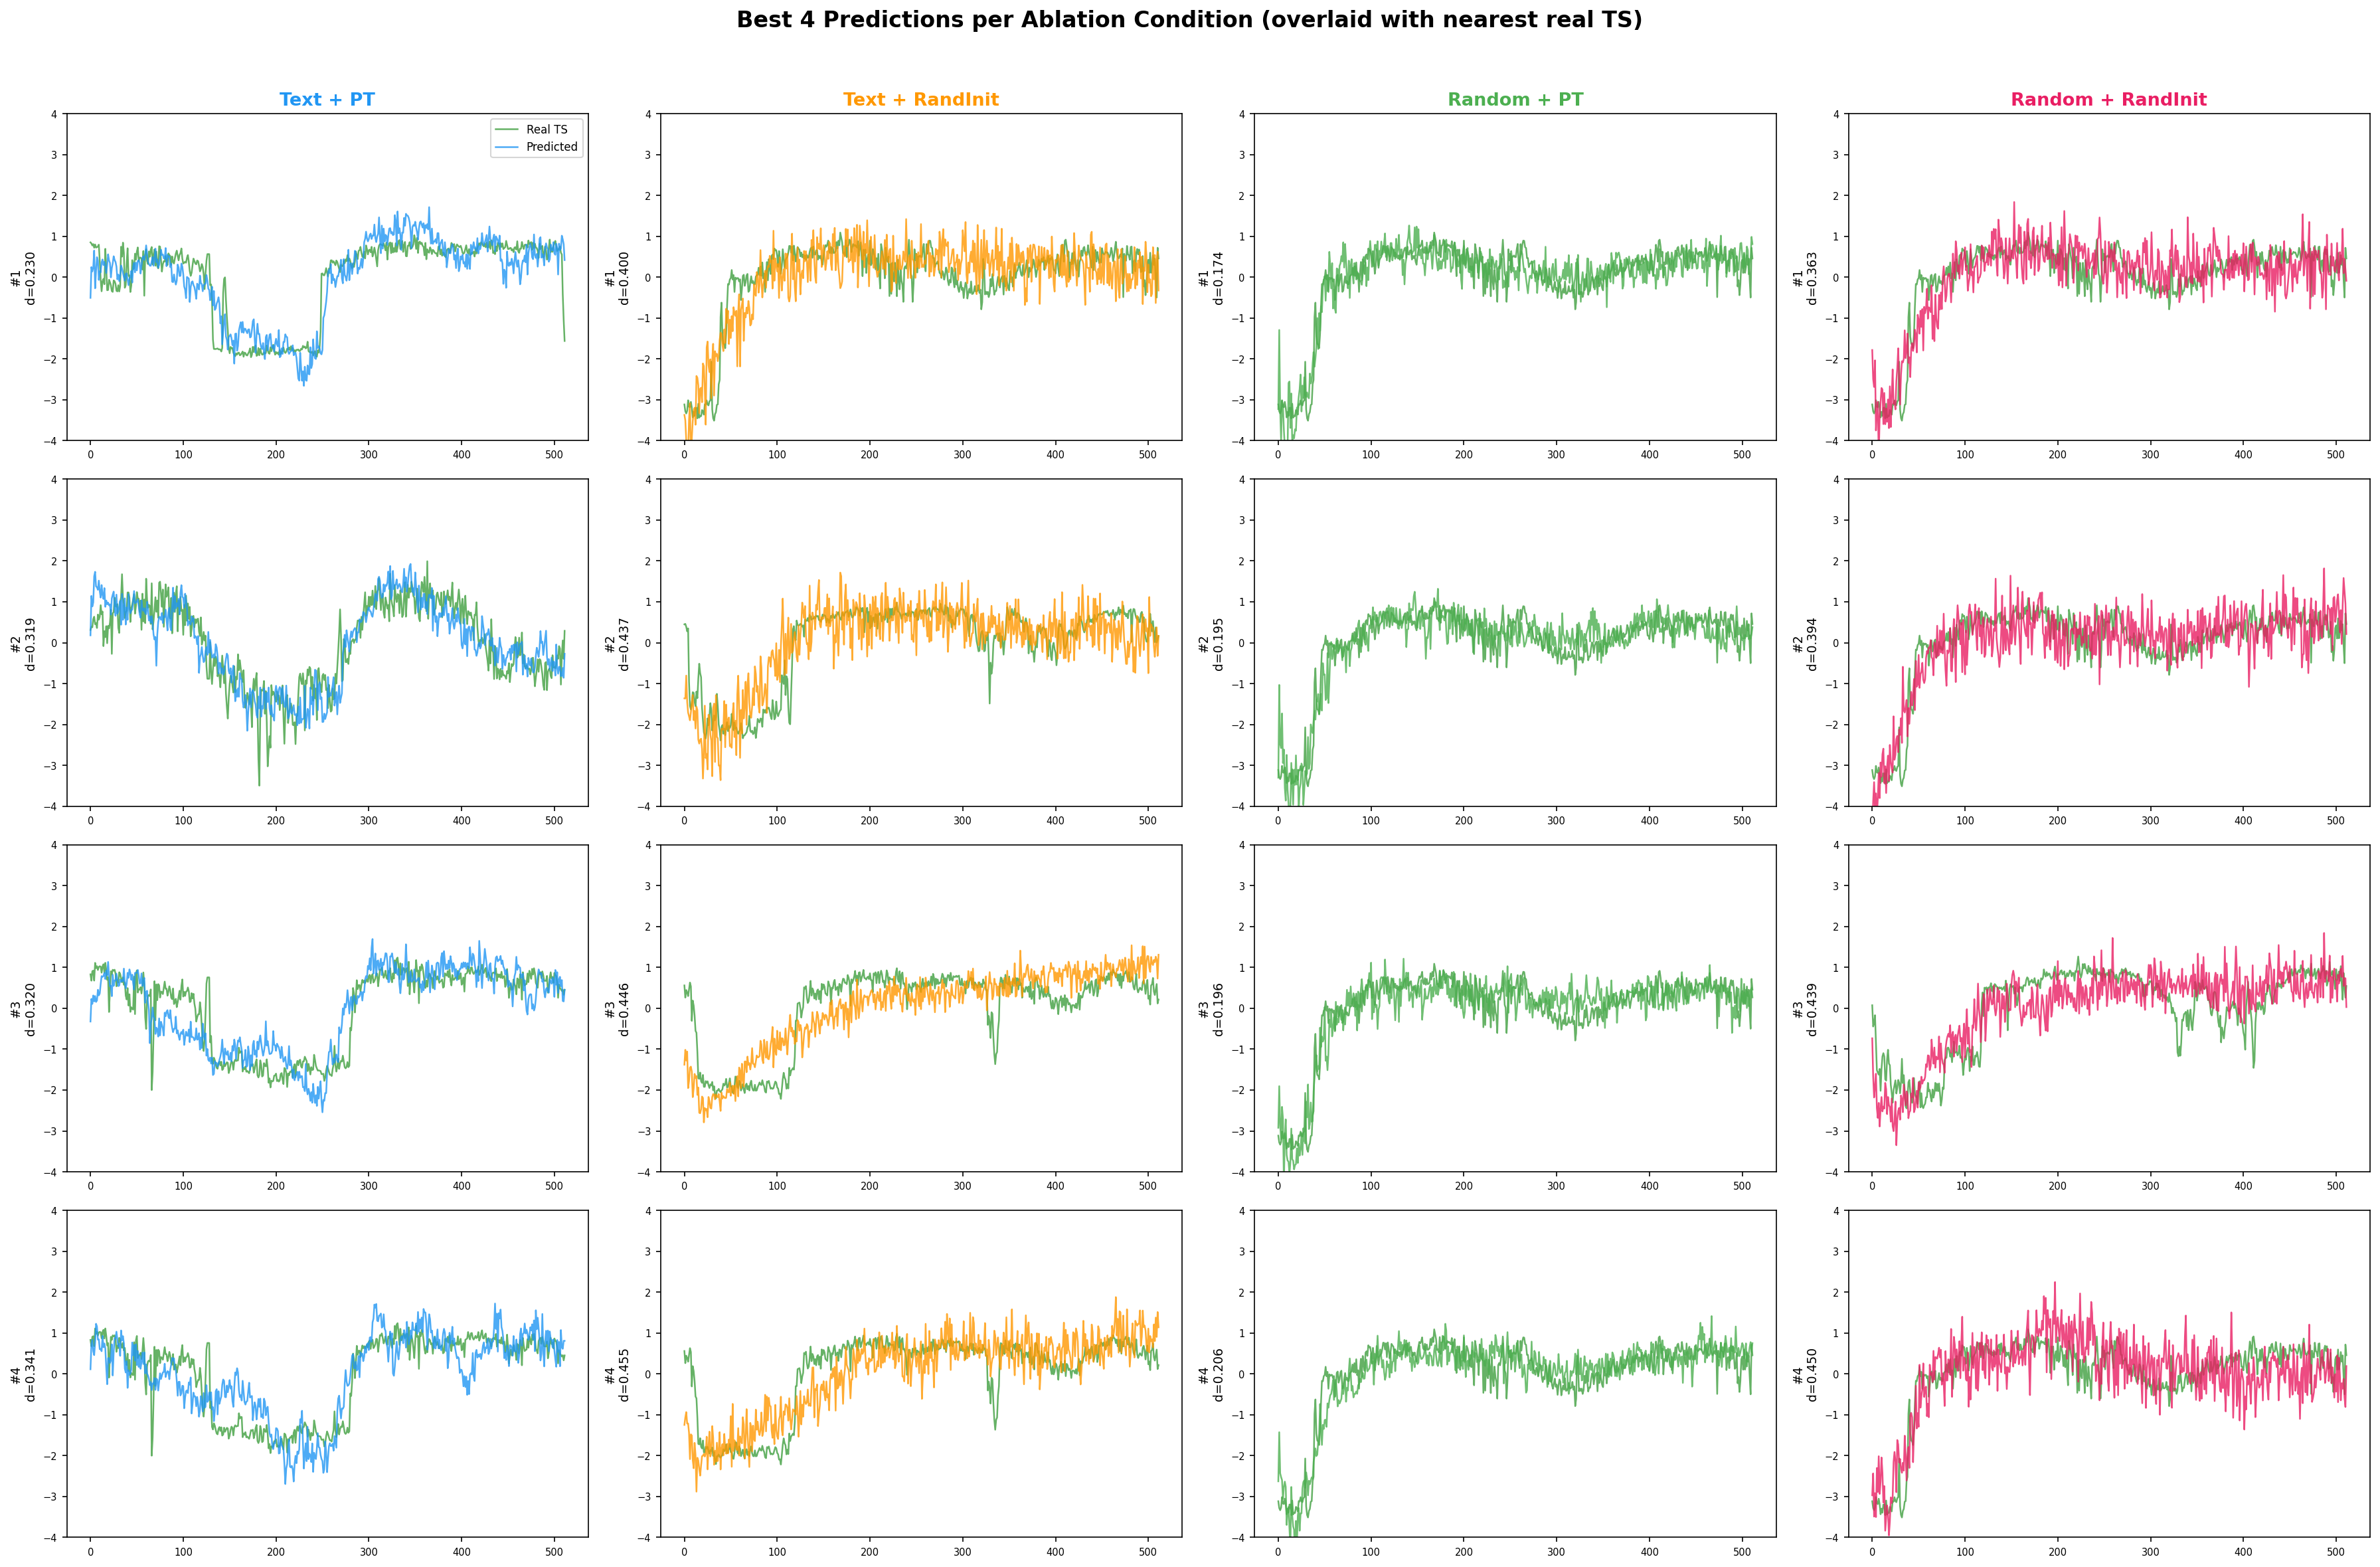
\includegraphics[width=\textwidth]{figures/fig_best4.png}
\caption{Best 4 predictions per ablation condition overlaid with their nearest real time series (green). text\_PT (blue, left) tracks the real TS closely across diverse shapes. rand\_PT (green, third column) produces near-identical outputs despite different inputs. RandInit models produce noisy, lower-quality matches.}
\label{fig:best4}
\end{figure}

\begin{figure}[t]
\centering
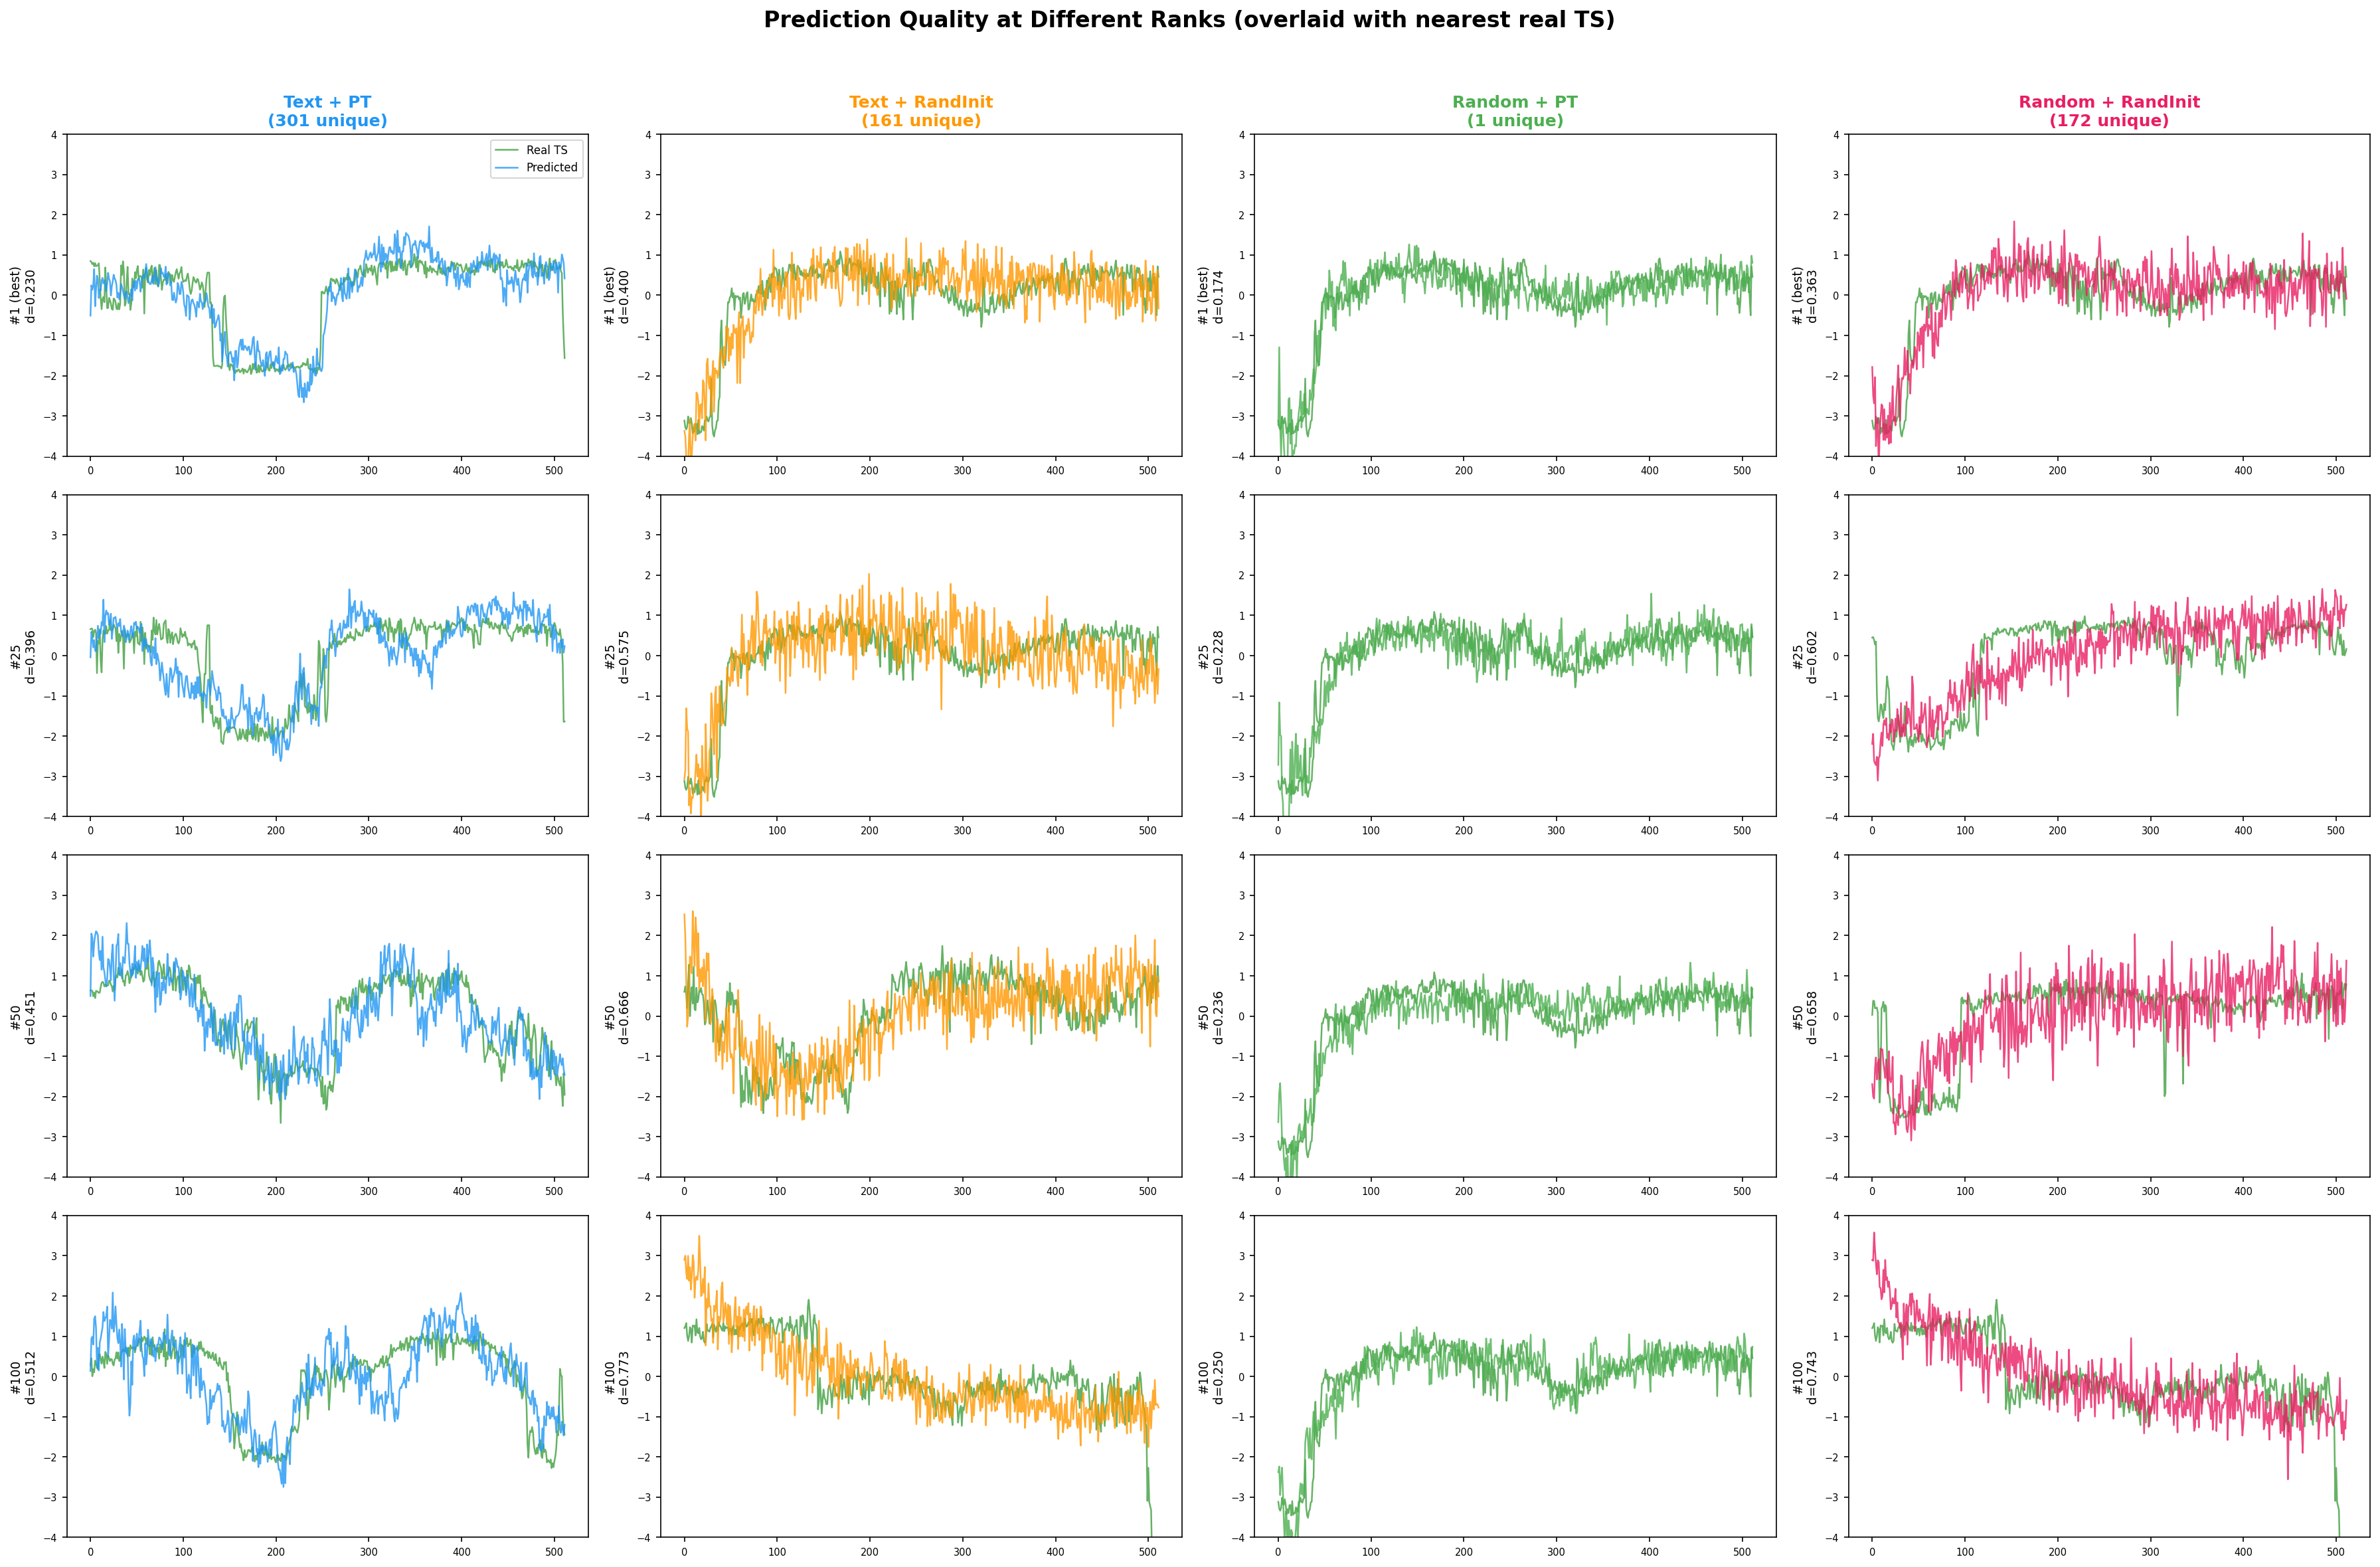
\includegraphics[width=\textwidth]{figures/fig_quality_levels.png}
\caption{Prediction quality at different ranks (\#1, \#25, \#50, \#100 best match) per ablation condition. text\_PT maintains good alignment even at rank \#100. rand\_PT has only 1 unique match (rows 2--4 blank).}
\label{fig:quality-levels}
\end{figure}

\begin{figure}[t]
\centering
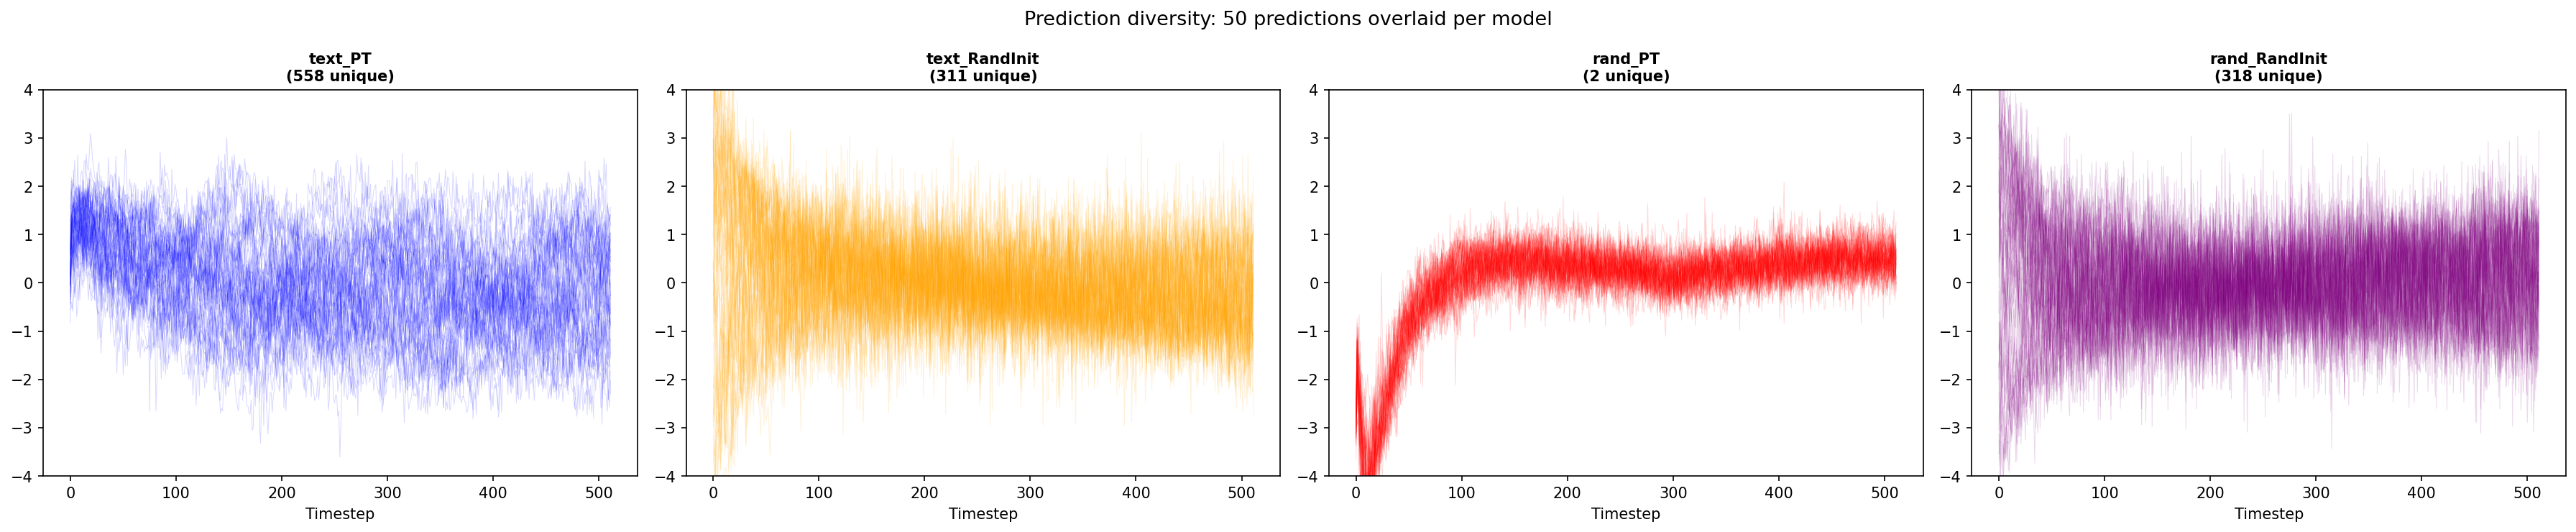
\includegraphics[width=\textwidth]{figures/fig_diversity.png}
\caption{50 random predictions overlaid per condition. text\_PT (top-left) shows rich waveform diversity. rand\_PT (bottom-left) collapses to a single shape. RandInit models (right column) show noisy but structurally limited variation.}
\label{fig:diversity}
\end{figure}

\begin{figure}[H]
\centering
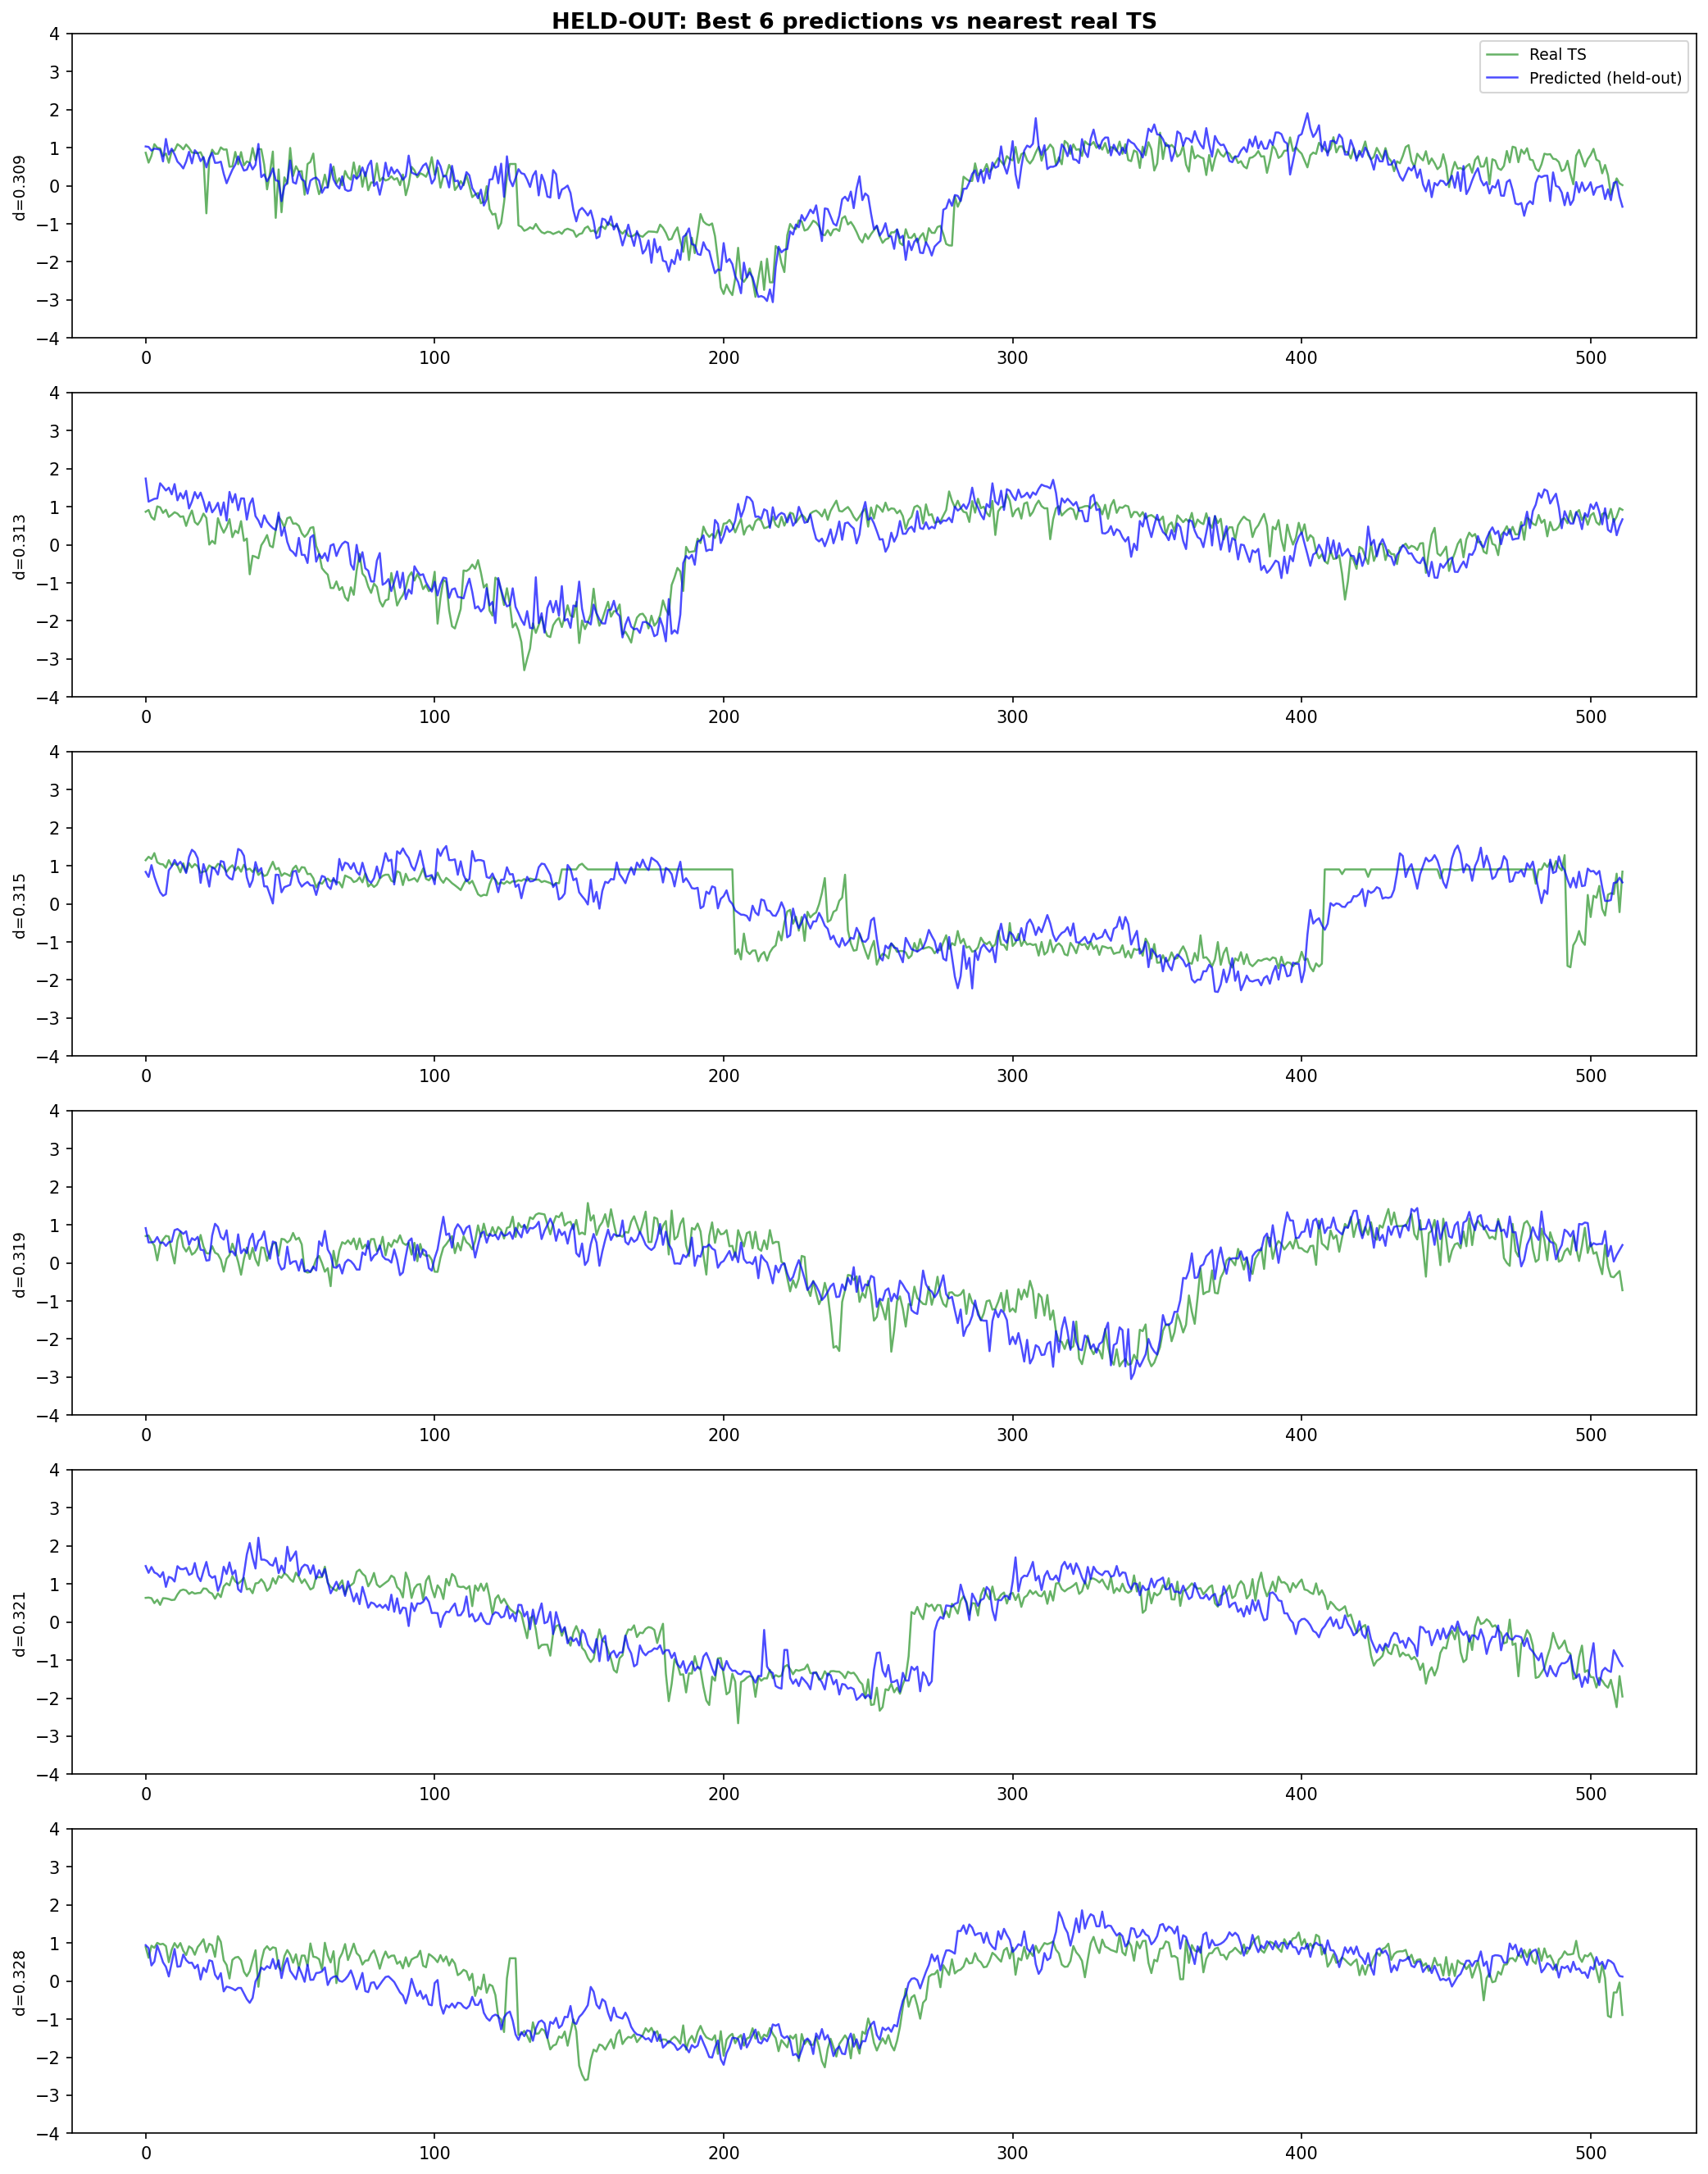
\includegraphics[width=\textwidth]{figures/fig_heldout_best6.png}
\caption{Best 6 held-out predictions (blue) vs.\ their nearest real time series (green). These sequences were never seen during mapper training, confirming generalization.}
\label{fig:heldout}
\end{figure}


% ════════════════════════════════════════════════════════════════
\section{Representation Geometry}

\subsection{Random Projection Baseline}

To determine whether the alignment between hidden states and time series is intrinsic to representation geometry or purely learned by the mapper, we evaluate \emph{random} linear projections with no training.

For each condition, we sample $R = 50$ random weight vectors $\bW_r \sim \mathcal{N}(0, I/D)$, project hidden states:
\begin{equation}
    \hat{y}_{i,t}^{(r)} = \bW_r \bh_{i,t}
\end{equation}
normalize predictions, and evaluate against the full 10{,}000 TS bank.

\begin{table}[H]
\centering
\begin{tabular}{lrrrr}
\toprule
Condition & NN Dist & Unique & Clusters & Entropy \\
\midrule
text\_PT & $1.36 \pm 0.30$ & $174 \pm 174$ & $12.5 \pm 8.2$ & $0.47 \pm 0.41$ \\
text\_RandInit & $1.04 \pm 0.02$ & $166 \pm 10$ & $17.1 \pm 0.8$ & $0.63 \pm 0.03$ \\
rand\_PT & $1.40 \pm 0.34$ & $106 \pm 157$ & $9.2 \pm 7.8$ & $0.32 \pm 0.37$ \\
rand\_RandInit & $1.10 \pm 0.02$ & $182 \pm 11$ & $17.5 \pm 0.7$ & $0.66 \pm 0.02$ \\
\bottomrule
\end{tabular}
\caption{Random projection baseline (mean $\pm$ std over 50 projections). PT models show enormous variance across projections; RandInit models are stable.}
\label{tab:random-proj}
\end{table}

The most striking result is the \emph{variance structure}: PT models exhibit standard deviations comparable to or exceeding their means (e.g., unique matches $174 \pm 174$ for text\_PT), while RandInit models show tiny relative variance ($166 \pm 10$).
This means PT representations contain \emph{rare, high-quality directions} that random projections occasionally hit, while RandInit representations are isotropic---all directions are equally mediocre.

Comparing to the trained mapper: text\_PT's trained mapper achieves NN $= 0.67$ with 686 unique matches, far surpassing any single random projection.
Training finds the optimal direction in a highly structured, anisotropic space.

\subsection{PCA Analysis}

We directly characterize representation geometry via PCA on flattened hidden states.
For each condition, we reshape the hidden state tensor $\mathbf{H} \in \R^{N \times T \times D}$ to $\mathbf{H}_{\text{flat}} \in \R^{NT \times D}$, subsample 50{,}000 rows, and fit randomized PCA with 500 components.

We report three metrics:

\paragraph{Effective rank.}
The exponential of the entropy of the normalized eigenvalue spectrum:
\begin{equation}
    r_{\text{eff}} = \exp\!\left(-\sum_{i=1}^{D} p_i \log p_i\right), \quad p_i = \frac{\lambda_i}{\Tr(\Sigma)} = \frac{\lambda_i}{\sum_{j=1}^D \lambda_j}
\end{equation}
where $\lambda_i$ are the eigenvalues of the covariance matrix and $\Tr(\Sigma) = \sum_j \lambda_j$ is the total variance (trace).
The effective rank ranges from 1 (all variance in one direction) to $D$ (uniform).

\paragraph{Participation ratio.}
\begin{equation}
    \text{PR} = \frac{\left(\sum_i \lambda_i\right)^2}{\sum_i \lambda_i^2}
\end{equation}
This measures how many eigenvalues contribute meaningfully to the total variance.

\paragraph{Cumulative variance.}
The number of PCA components needed to explain a given fraction of total variance.

\begin{table}[H]
\centering
\begin{tabular}{lrrrrrr}
\toprule
Condition & Mean Var & Eff.\ Rank & PR & 90\% & 95\% \\
\midrule
text\_PT & 104.4 & 5.6 & 1.5 & 60 & 315 \\
text\_RandInit & 3.8 & 431.3 & 138.6 & 421 & 500+ \\
rand\_PT & 93.1 & 2.8 & 1.3 & 2 & 91 \\
rand\_RandInit & 3.9 & 585.3 & 207.6 & 500+ & 500+ \\
\bottomrule
\end{tabular}
\caption{Hidden state geometry. PT models concentrate variance into $\sim$3--6 effective dimensions; RandInit models spread across 400--600. ``90\%'' / ``95\%'' = number of PCs for that cumulative variance.}
\label{tab:pca}
\end{table}

\textbf{PT representations are extremely anisotropic.}
For text\_PT, the first principal component alone captures 81.5\% of total variance, and the effective rank is just 5.6 out of $D = 28{,}672$.
For rand\_PT, the concentration is even more extreme: 89.2\% in the first component, effective rank 2.8.

\textbf{RandInit representations are near-isotropic.}
text\_RandInit and rand\_RandInit have effective ranks of 431 and 585 respectively, with no dominant eigenvalues (the largest explains only 1.7--3.0\% of variance).

\begin{figure}[H]
\centering
\includegraphics[width=\textwidth]{figures/fig_pca_spectrum.png}
\caption{PCA eigenvalue spectrum (top 100 components). Left: linear scale showing the extreme first eigenvalue of PT models. Right: log scale revealing the spectral structure across all conditions.}
\label{fig:pca}
\end{figure}

\begin{figure}[H]
\centering
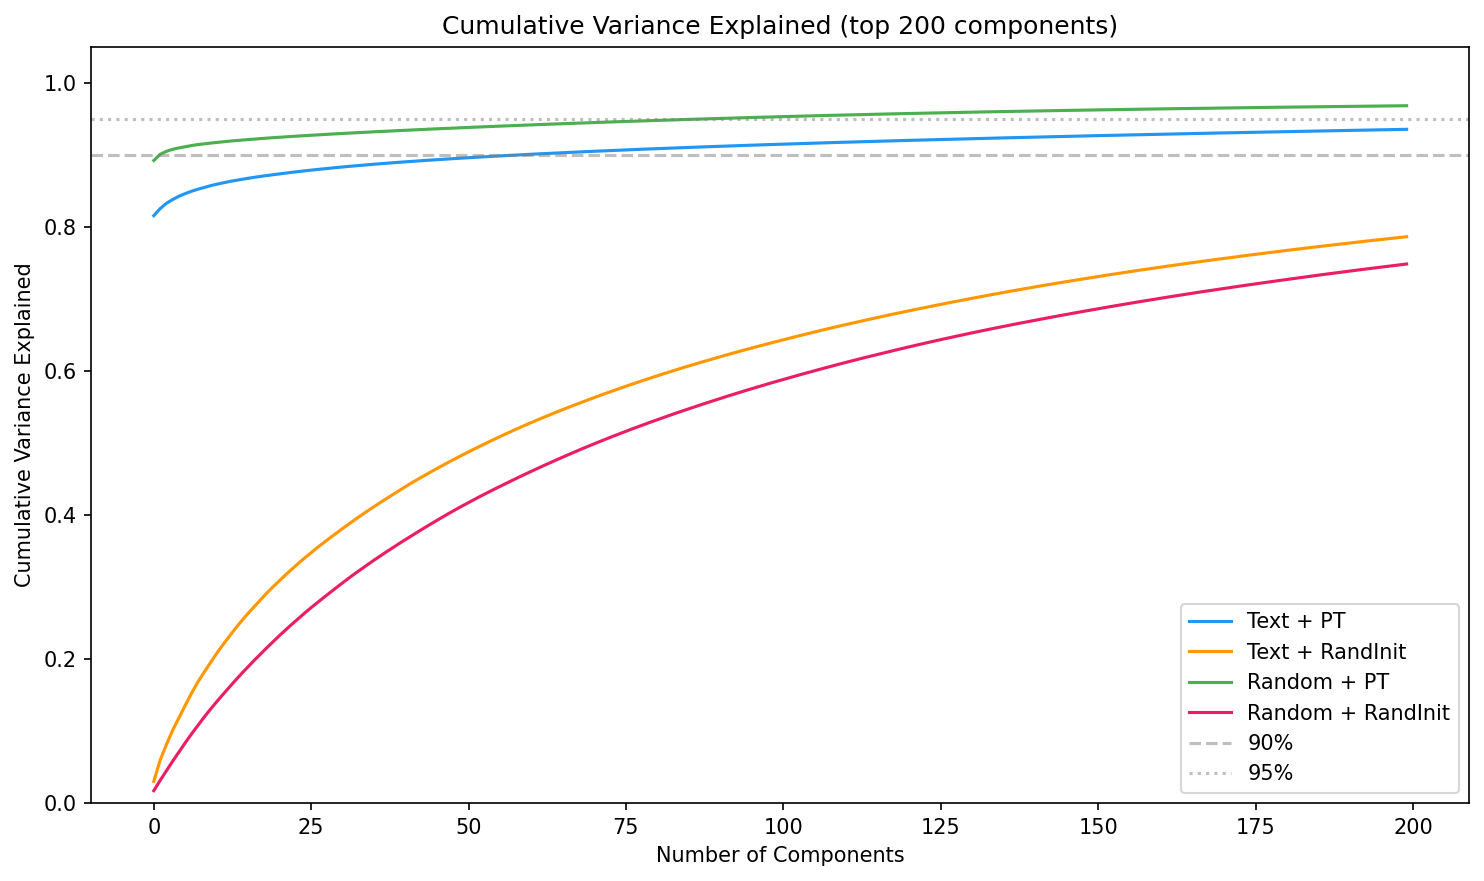
\includegraphics[width=0.7\textwidth]{figures/fig_cumvar.png}
\caption{Cumulative variance explained. PT models reach 90\% with 2--60 components; RandInit models require 420+ components and still don't reach 95\% within 500.}
\label{fig:cumvar}
\end{figure}

\subsection{Interpretation}

The anisotropy of PT representations provides a unified explanation for several observations:

\begin{enumerate}[nosep]
    \item \textbf{Why linear decoding works}: The pretrained model compresses its representation into a low-dimensional manifold. A linear map can extract useful signal because the relevant information lies in a few accessible directions.
    \item \textbf{Why random projections are unstable}: With effective rank $\sim$5 in a 28{,}672-dimensional space, a random direction has probability $\sim$5/28{,}672 $\approx$ 0.02\% of aligning with the important subspace. Most random projections miss entirely; rare ones hit.
    \item \textbf{Why training matters}: The EM-style training procedure finds the optimal direction in this low-dimensional subspace---something random projections cannot reliably do.
    \item \textbf{Why RandInit is mediocre but stable}: With isotropic geometry (effective rank $\sim$500), all directions are equivalent. Training cannot find a better direction because none exists.
\end{enumerate}

% ════════════════════════════════════════════════════════════════
\section{Spectral Properties}

\subsection{Power Spectrum Comparison}

We compare the frequency content of decoded predictions against real time series.
For each sequence $\by \in \R^T$, we compute the normalized PSD:
\begin{equation}
    \PSD(\by) = \frac{|\FFT(\by)|^2}{\sum_f |\FFT_f(\by)|^2} \in \R^{T/2+1}
\end{equation}
and average across sequences.
We measure alignment via $L_2$ distance and KL divergence between mean PSDs, and decompose energy into frequency bands.

\begin{table}[H]
\centering
\begin{tabular}{lrrrrr}
\toprule
Condition & PSD $L_2$ & KL Div & Low (0--10\%) & Mid (10--50\%) & High (50--100\%) \\
\midrule
text\_PT & 0.228 & 0.267 & 90.1\% & 6.6\% & 3.3\% \\
text\_RandInit & 0.274 & 0.431 & 58.4\% & 19.5\% & 22.1\% \\
rand\_PT & \textbf{0.120} & \textbf{0.125} & 89.8\% & 5.8\% & 4.5\% \\
rand\_RandInit & 0.264 & 0.443 & 55.3\% & 21.0\% & 23.7\% \\
\midrule
\textbf{Real TS} & --- & --- & 79.2\% & 13.7\% & 7.2\% \\
\bottomrule
\end{tabular}
\caption{Spectral alignment. PT models concentrate energy in low frequencies, closely matching real TS. RandInit models produce spectrally flat (noisy) outputs.}
\label{tab:spectral}
\end{table}

\begin{figure}[H]
\centering
\includegraphics[width=\textwidth]{figures/fig_psd.png}
\caption{Mean PSD: predictions vs.\ real TS. Left: linear scale. Right: log scale. PT models (blue, green) match the low-frequency dominance of real TS (black). RandInit models (orange, pink) are spectrally flat.}
\label{fig:psd}
\end{figure}

\begin{figure}[H]
\centering
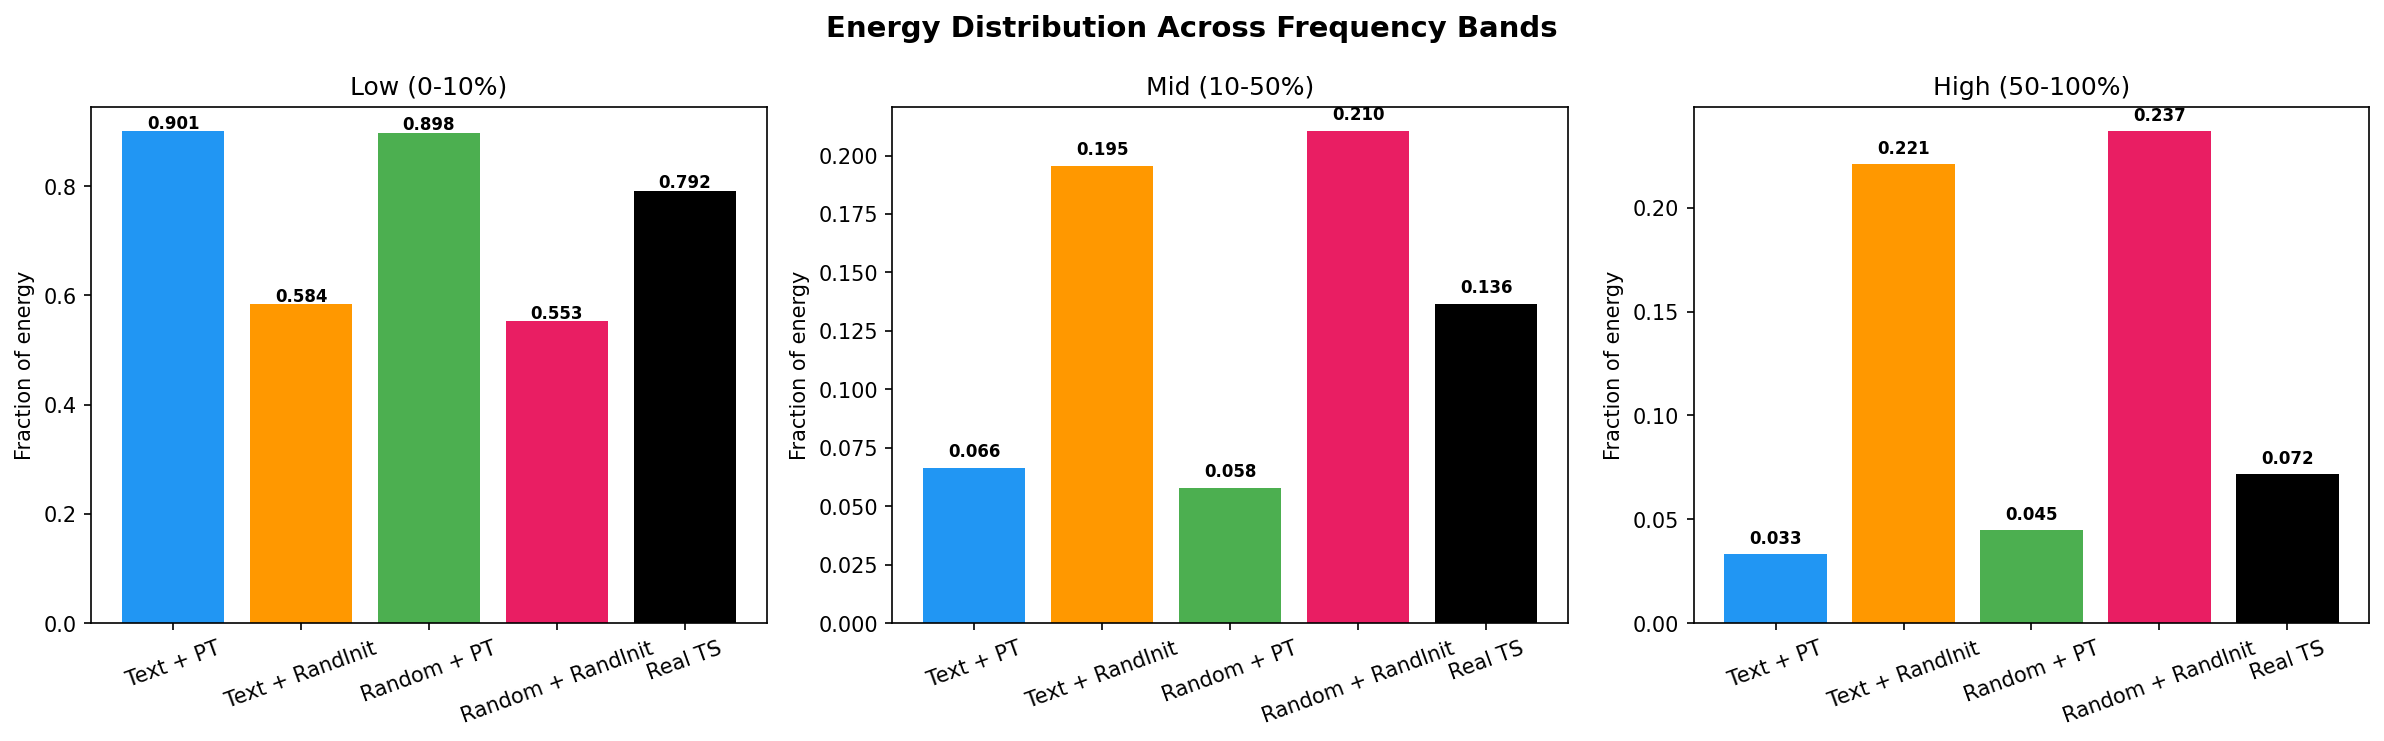
\includegraphics[width=\textwidth]{figures/fig_freq_bands.png}
\caption{Energy distribution across frequency bands for each condition and real TS.}
\label{fig:freq-bands}
\end{figure}

\subsection{Interpretation}

PT models produce \emph{smooth, low-frequency-dominated} outputs (90\% low-band energy) that closely match the spectral profile of real time series (79\% low-band).
RandInit models produce spectrally flat, noisy outputs (55--58\% low-band, 22--24\% high-band).

Notably, rand\_PT achieves the \emph{best} spectral alignment (PSD $L_2 = 0.120$) despite collapsing to only 1--4 unique outputs.
This demonstrates that spectral realism alone is insufficient---it can be achieved by mode-collapsing to a single representative waveform.
Only text\_PT achieves both spectral alignment \emph{and} output diversity.

% ════════════════════════════════════════════════════════════════
\section{Synthesis}

\subsection{Mechanism}

Our results support the following mechanistic model of how linear decoding works:

\begin{enumerate}[nosep]
    \item \textbf{Pretraining compresses representations} into a low-dimensional subspace (effective rank $\sim$3--6) dominated by 1--2 principal directions.
    \item \textbf{This subspace encodes smooth temporal dynamics}: the autoregressive training objective induces representations that vary smoothly along the sequence dimension, producing low-frequency-dominated outputs when linearly projected.
    \item \textbf{Text input traverses the manifold}: different text sequences move the hidden state through different trajectories on this low-dimensional manifold, enabling diverse outputs.
    \item \textbf{Linear decoding projects these trajectories} into one-dimensional time series that resemble real-world temporal patterns.
\end{enumerate}

\subsection{Why Each Component Is Necessary}

\begin{itemize}[nosep]
    \item \textbf{Trained weights}: Create the low-dimensional manifold with smooth temporal dynamics. Without training, representations are isotropic and all projections yield noise.
    \item \textbf{Meaningful text}: Drives the hidden state through varied trajectories on the manifold. Random tokens produce uniform hidden states that collapse to a single output.
    \item \textbf{The linear map}: Extracts the right direction in the low-dimensional subspace. Random projections occasionally find good directions but cannot do so reliably in a 28{,}672-dimensional space with effective rank $\sim$5.
\end{itemize}

\subsection{Failure Modes}

\begin{itemize}[nosep]
    \item \textbf{Mode collapse}: The primary failure mode. The EM objective naturally rewards matching the most common TS pattern. Mitigated by the PSD diversity penalty ($\lambda = 0.5$), but not eliminated.
    \item \textbf{Seed sensitivity}: Results vary across random seeds (601--883 unique matches across seeds 0--4). Some seeds collapse entirely, likely due to early EM assignments trapping the mapper in a local minimum.
    \item \textbf{Over-smoothing}: PT predictions concentrate 90\% of energy in low frequencies (vs.\ 79\% for real TS), under-representing mid/high frequency variation.
\end{itemize}

% ════════════════════════════════════════════════════════════════
\section{Conclusion}

We have shown that pretrained language models encode latent temporal structure that can be linearly decoded into realistic time series without any paired supervision.
This structure is:
\begin{itemize}[nosep]
    \item \textbf{Low-dimensional}: effective rank $\sim$3--6 in a 28{,}672-dimensional space, with 80--89\% of variance in a single direction.
    \item \textbf{Spectrally aligned}: decoded outputs match the low-frequency dominance of real time series (90\% vs.\ 79\% low-band energy).
    \item \textbf{Dependent on both training and semantics}: neither trained weights alone nor meaningful text alone produces diverse, high-quality outputs.
\end{itemize}

These findings suggest that autoregressive language pretraining induces a latent dynamical system in representation space---one whose temporal structure is rich enough to be linearly projected into observable time series signals.
The extreme anisotropy of pretrained representations (effective rank $\sim$5 despite 28{,}672 dimensions) implies that language models learn to compress sequential information into a remarkably compact subspace, and it is this compression that enables---and constrains---cross-modal transfer.

% ════════════════════════════════════════════════════════════════
\appendix
\section{Additional Training Details}

\paragraph{Infrastructure.}
All experiments were conducted on a machine with 4$\times$ NVIDIA RTX 5090 (32\,GB each) and 755\,GB RAM.
Hidden state extraction (28 layers, 2000 sequences) takes $\sim$3 minutes.
Mapper training (100 epochs, batch 32, concat layers) takes $\sim$45 minutes.
NN evaluation ($N$ predictions $\times$ 10{,}000 TS bank) takes $\sim$8 minutes.

\paragraph{Hidden state storage.}
Concatenated hidden states for 2000 sequences ($2000 \times 512 \times 28{,}672$ in float16) require $\sim$55\,GB.
We store these as float16 numpy memmaps on disk, loading batches to float32 on GPU during training.

\paragraph{Seed stability.}
We tested 5 random seeds (0--4) with the text\_PT concatenated configuration.
Unique matches ranged from 601 to 883 across seeds, with seed 2 exhibiting partial collapse.
Seed 1 was selected for all subsequent experiments based on stability.

\section{Additional Results}

\begin{figure}[H]
\centering
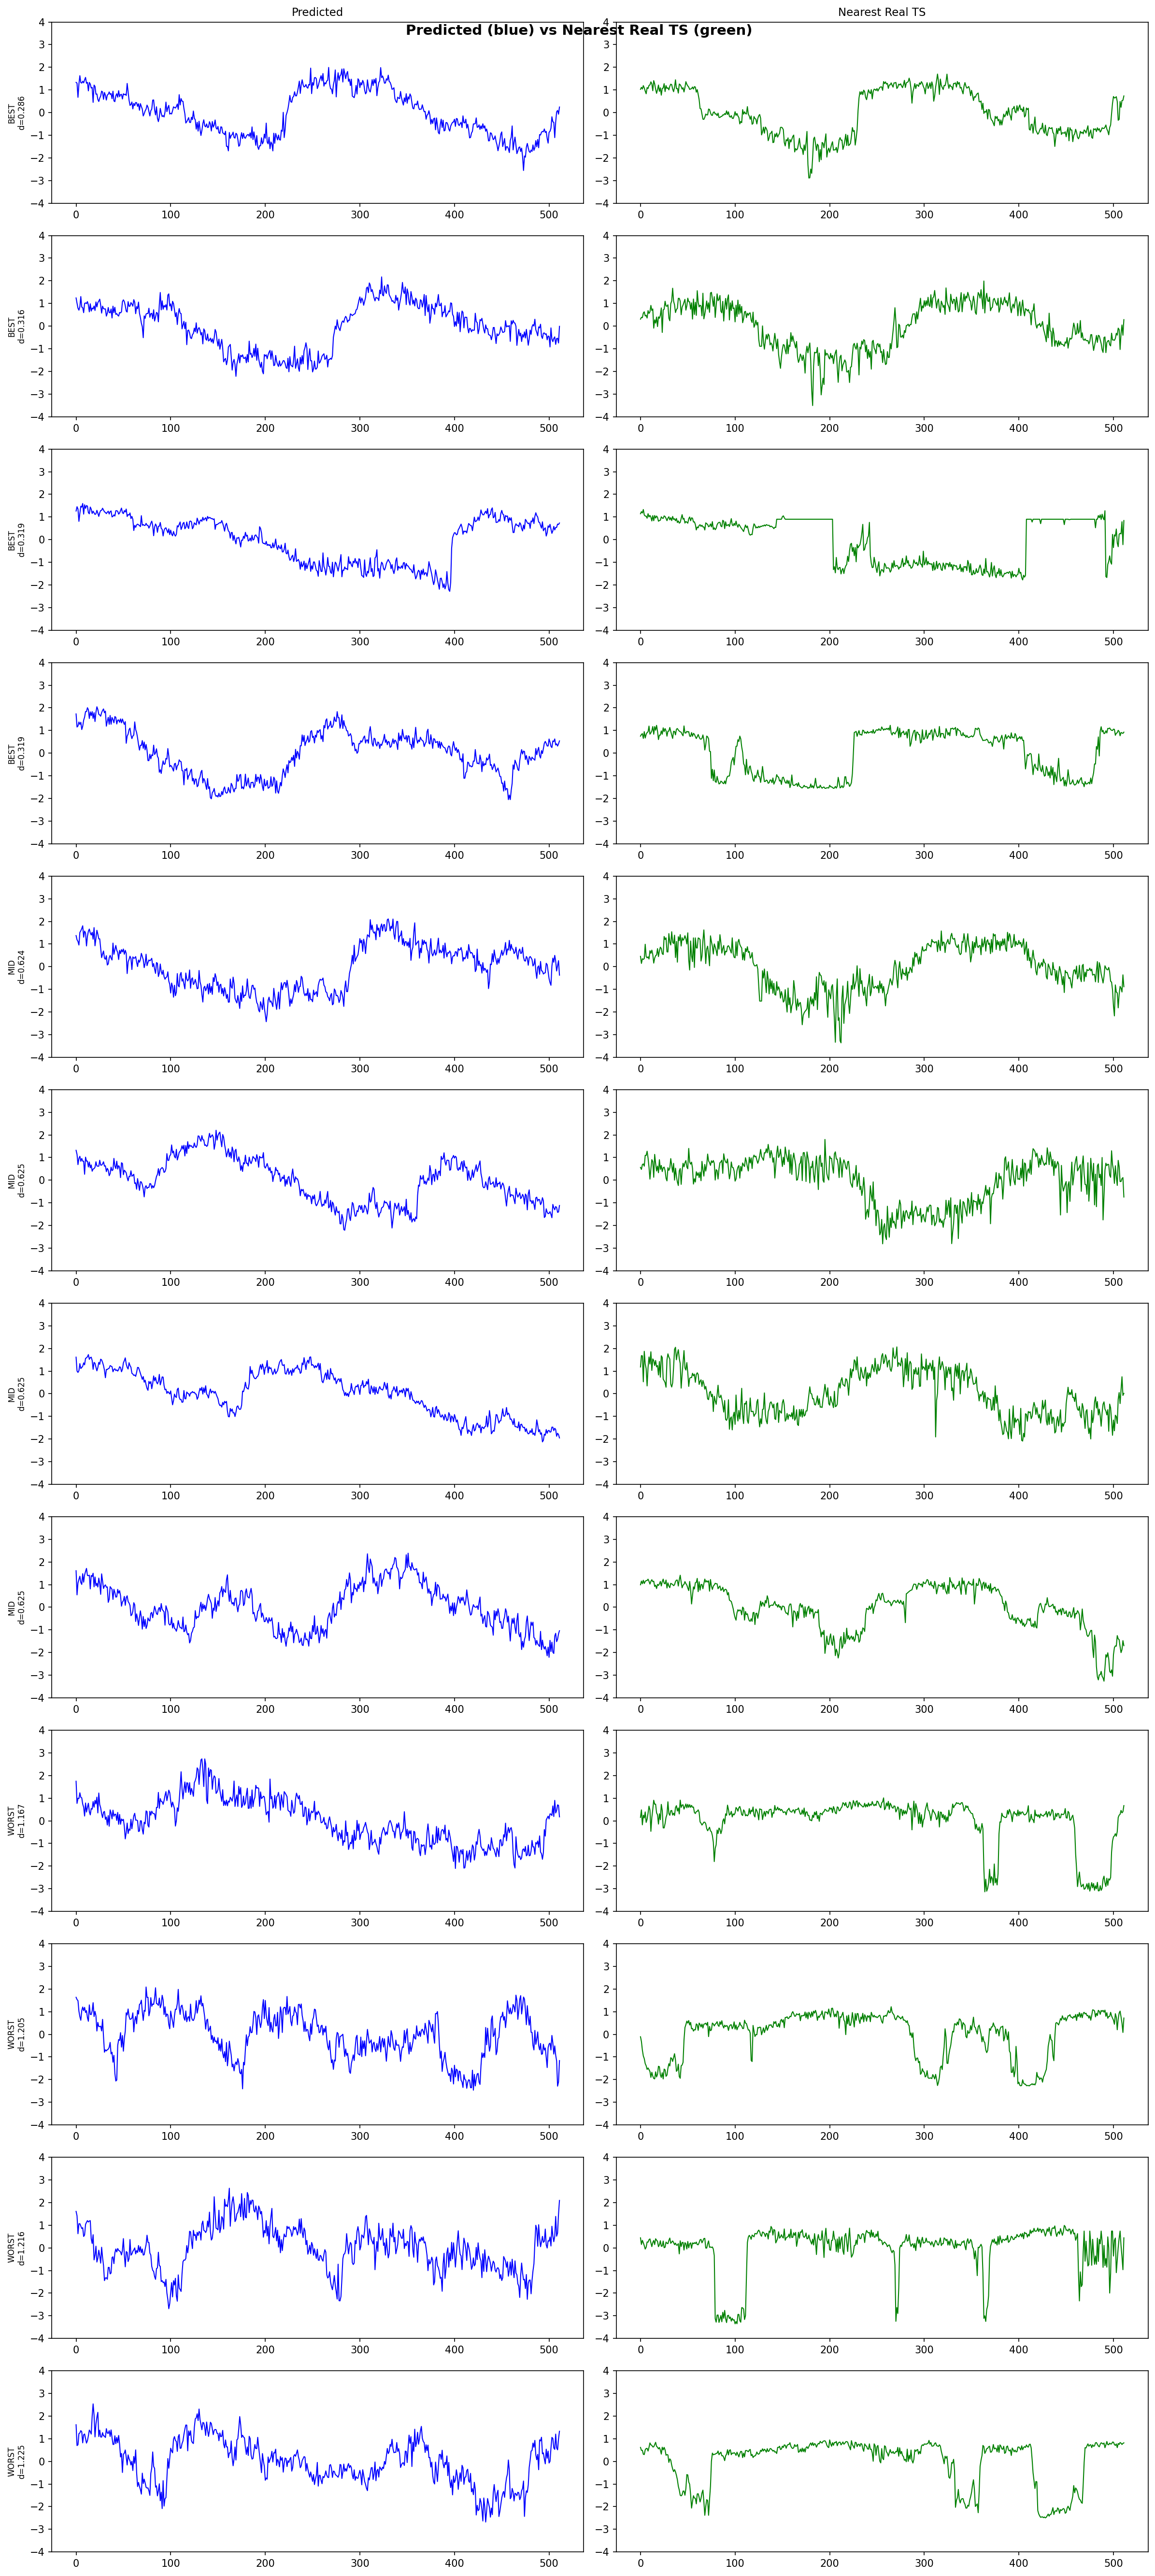
\includegraphics[width=\textwidth]{figures/fig_quality_grid.png}
\caption{Quality grid for text\_PT: best, middle, and worst predictions (left) vs.\ their nearest real time series (right). Even mid-quality predictions capture the broad temporal shape.}
\label{fig:quality-grid}
\end{figure}

\begin{figure}[H]
\centering
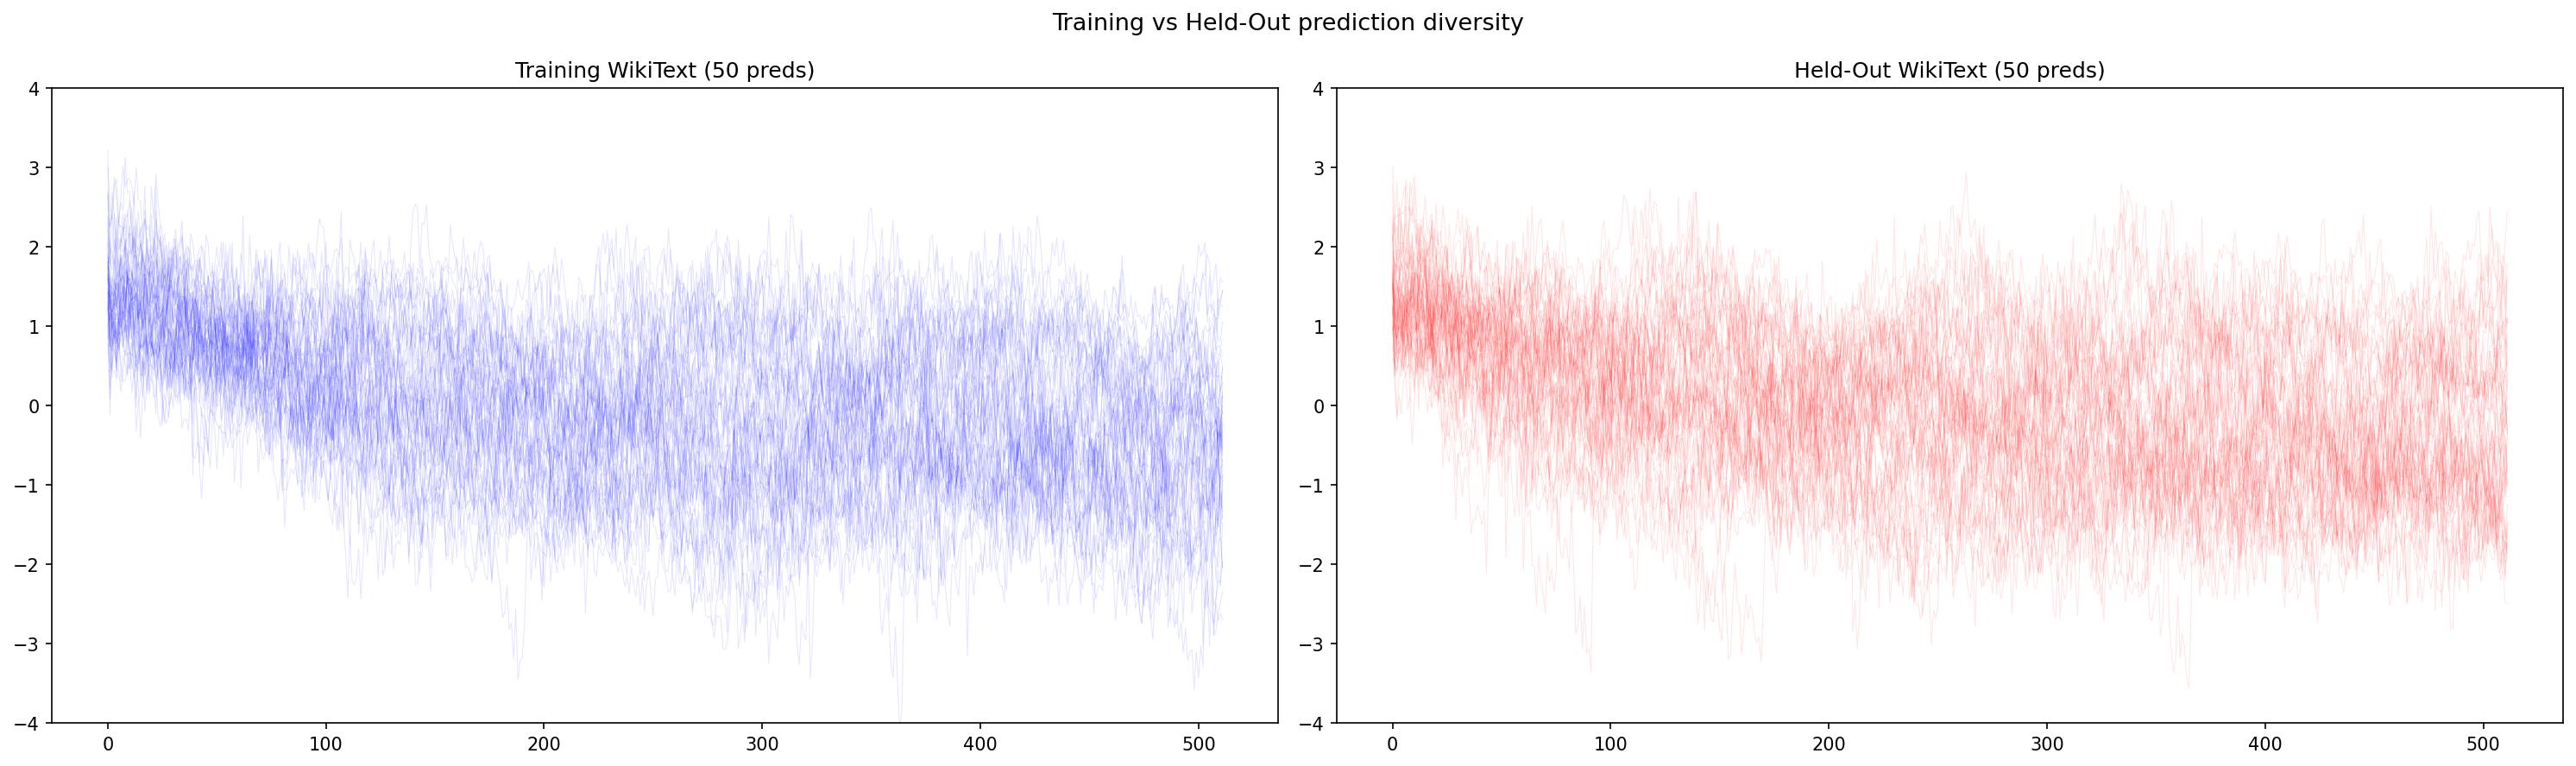
\includegraphics[width=\textwidth]{figures/fig_train_vs_held.png}
\caption{Training (left) vs.\ held-out (right) prediction diversity for text\_PT. Both show similar waveform variety, confirming generalization.}
\label{fig:train-held}
\end{figure}

\begin{figure}[H]
\centering
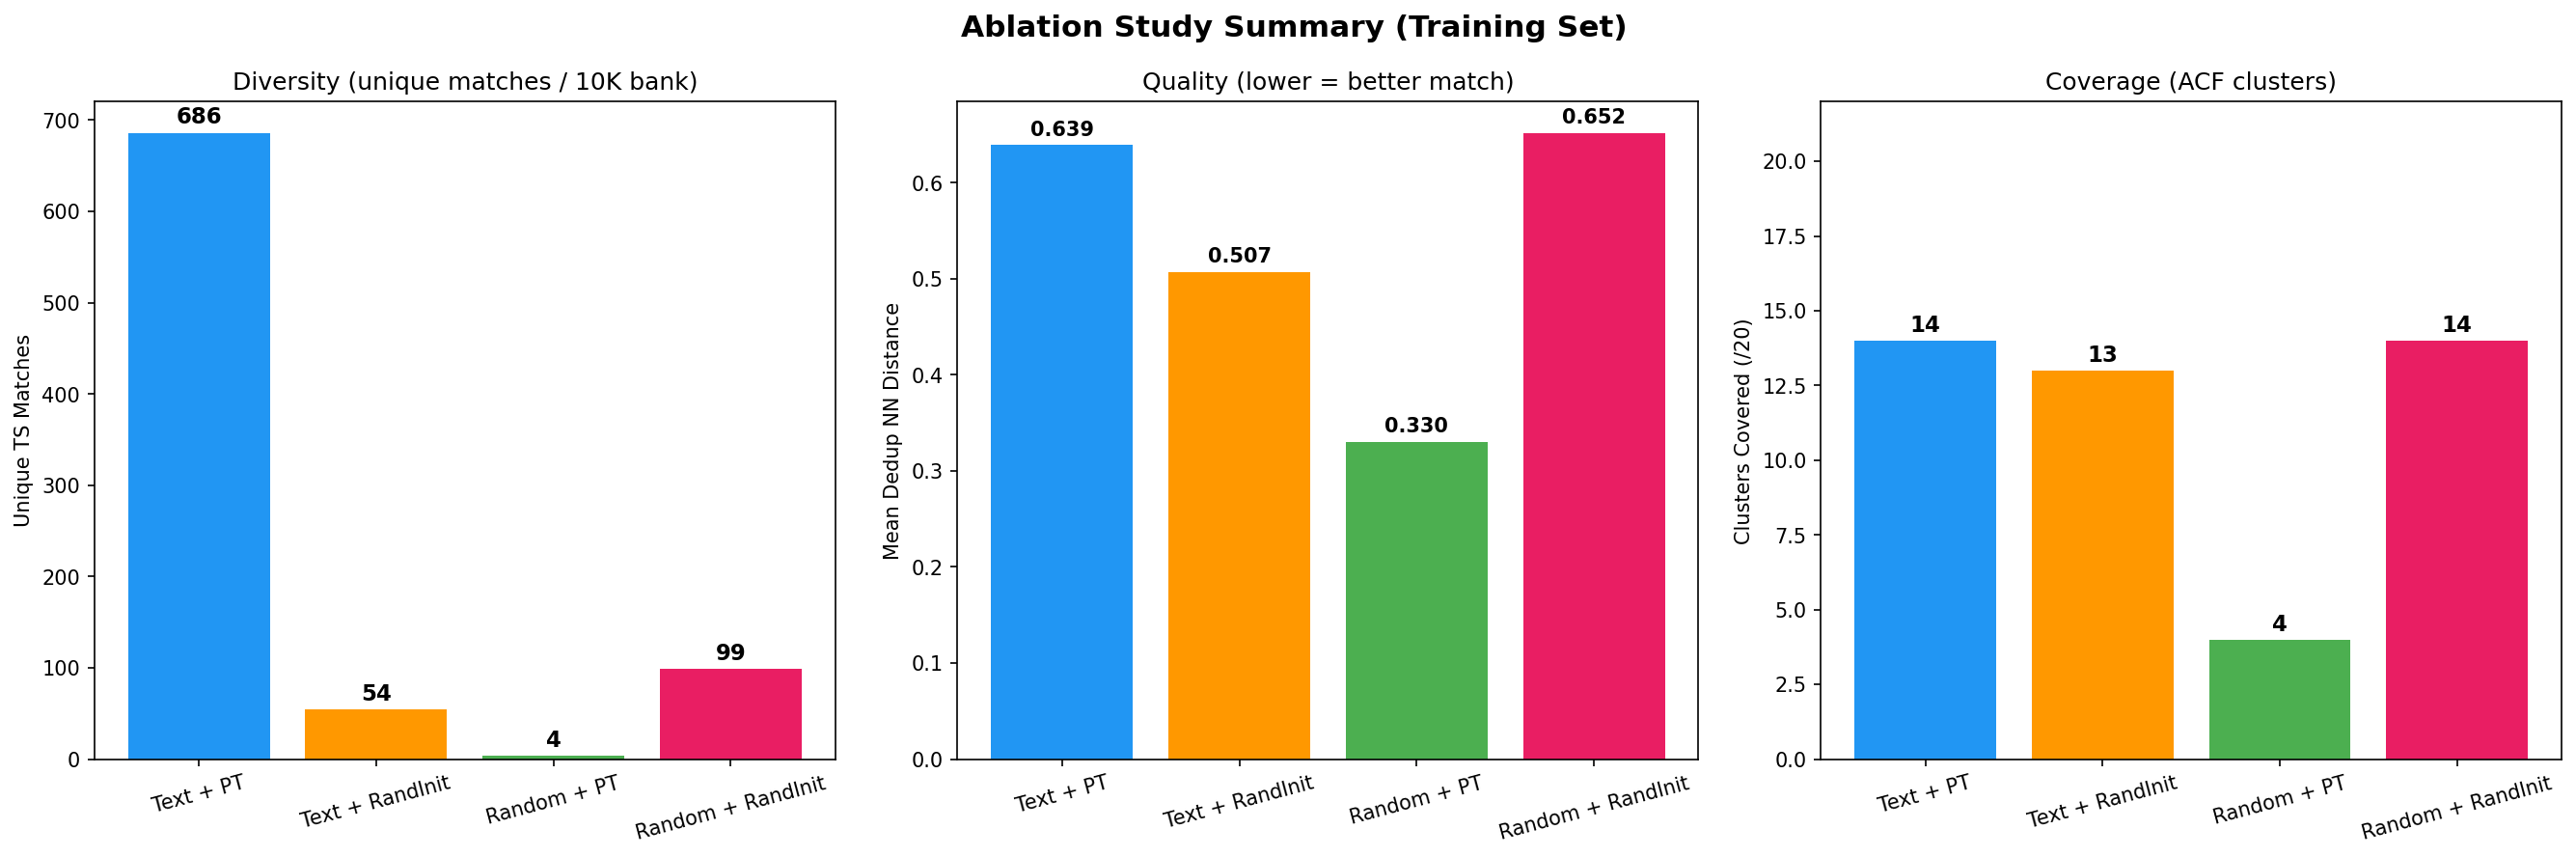
\includegraphics[width=0.6\textwidth]{figures/fig_ablation_summary.png}
\caption{Summary of ablation study: diversity (unique matches), quality (dedup NN distance), and cluster coverage across all four conditions.}
\label{fig:ablation-summary}
\end{figure}

\end{document}
